\chapter{OSTES Validation}
\label{chap:OSTESValid}

The OSTES algorithm was tested on both synthetic and real data. Synthetic data were generated from spectral and climatological  libraries such that they cover many possible scenes and conditions. These data were simulated as would be acquired with ASTER, AHS and TASI sensor. The OSTES was further tested on a real data. For this purpose were chosen image data acquired by ASTER and TASI sensor. The ASTER image data include water bodies of the Caspian Sea and Lake Baikal. The TASI image data contain urban areas of city of Brno. 

\section{Synthetic Data}

\subsection*{Imaging Systems}

Synthetic data are intended to cover many possible situations of acquiring thermal data. Therefore three different sensor architectures were chosen to test the OSTES algorithm and compare the results with the TES algorithm.

From the wide range of airborne sensors operating in the TIR region two are chosen as examples: the AHS operated by Spanish Institute of Aeronauics (INTA) and developed by ArgonST (Fairfax, USA), and the TASI sensor. These sensors offer data of great importance in applications. Notable studies include areas of
mineral mapping \cite{NK14}, 
soil moisture estimation \cite{SF12}, 
urban studies \cite{SO12},
soil organic carbon estimation \cite{PC14} and
crop water stress characterization \cite{PP12},
among others.

\begin{figure}[!t]
\centering
\includegraphics[width=0.9\linewidth]{pics/Chapter_04/response_functions_all.pdf}
\vspace{1.5 em}
\caption{Response functions for ASTER, AHS and TASI sensors. The ASTER Band Numbers are shown above the ASTER response functions.}
\label{fig:ResponseFunctions}
\end{figure}
 
The above-mentioned airborne sensors were chosen together with the ASTER sensor to analyze the performance of the OSTES algorithm. ASTER consists of 15 bands of which 5 are situated in TIR region with Noise Equivalent Temperature difference $\mathrm{(NE\Delta T)} \approx 0.3\,\mathrm{K}$. The spatial resolution of the TIR bands is $90\,\mathrm{m}$. The AHS sensor has been fully operational from 2005 \cite{FM05}. Its sensor operates in 80 spectral bands where the last 10 bands cover atmospheric window from 8 to $\SI{13}{\micro\meter}$ \cite{SJ06}. The AHS TIR bands have a  {Full Width at Half Maximum} $\mathrm{(FWHM)} \approx \SI{0.5}{\micro\meter}$ with $\mathrm{NE\Delta T} \approx 0.5\,\mathrm{K}$. The third sensor we will consider is the TASI sensor. It contains 32 bands all of which are in the TIR region. Bands are situated in the 8 to $\SI{11.5}{\micro\meter}$ region and have a $\mathrm{FWHM} \approx \SI{0.11}{\micro\meter}$ with $\mathrm{NE\Delta T} \approx 0.1\,\mathrm{K}$. The response functions of these sensors are depicted in Figure \ref{fig:ResponseFunctions}.

\subsection*{Data Set}

A data set of 6588 samples was artificially created to compare the performance of the TES and OSTES algorithms. Samples include 108 different natural surfaces chosen from ASTER spectral library \cite{BH09} at different temperatures coupled with 61 different atmospheric conditions taken from TIGR (TOVS Initial Guess Retrieval) database \cite{CS85, CC98}. Sample temperatures range from \SI{244}{\kelvin} to \SI{310}{\kelvin}. In order to simulate real conditions, every sample at a certain temperature is coupled with a certain type of atmosphere. The chosen atmospheres represent a variety of possible conditions within polar, mid-latitude and tropical airmasses. These samples were processed to land-leaving and downwelling radiance, as standard TES algorithm input, and they were transformed to band-effective quantities with respect to the ASTER, AHS and TASI response functions. Samples were passed to the algorithms individually.

\begin{table}[!t]
\vspace{0.5em}
\footnotesize
\centering
\begin{tabular}{lcccc}
\toprule
Sensor & $a$ & $b$ & $c$ & $r^2$\\ \hline
ASTER & $0.994$ & $-0.687$ & $0.737$ & $0.983$ \\
AHS & $1.000$ & $-0.782$ & $0.817$ & $0.994$ \\
TASI & $1.001$ & $-0.737$ & $0.760$ & $0.997$ \\
\bottomrule
\end{tabular}
\vspace{1.5 em}
\caption{Regression coefficients of $\varepsilon_\mathrm{min} = a + b\:\mathrm{MMD}^c$ and coefficients of determination $r^2$.}
\label{table:MMDcoef}
\normalsize
\end{table}

\newpage
Simulated data for the ASTER sensor were processed with the current implementation of TES, as it is used for generation of ASTER standard products AST\_05 and AST\_08 \cite{B15}. The version of the original TES algorithm in cases of AHS and TASI sensors was implemented in a manner similar to that described in \cite{JS12}. In addition, the implementation omits the $\varepsilon_\mathrm{max}$ refinement for emissivities with low spectral contrast. The OSTES was applied to all sensors as it is described in section \ref{sec:TES}.

Let us remind the reader that the regression coefficients in the (\ref{eq:MMD}) needs to be refined for each sensor with respect to its response functions. The regression coefficients in (\ref{eq:MMD}) were recomputed for AHS and TASI sensors using their respective response functions. In both cases the regression was performed on a set of 108 spectra chosen from same categories and library as in the ASTER case. The coefficients for different sensors are shown in the Table~\ref{table:MMDcoef}.

\subsection*{Validation}

Samples were passed to the TES and OSTES algorithms and the temperature and emissivity results were compared with true values. We divide the results into two groups according to the emissivity spectral contrast. For each sensor type we determined a threshold for Maximum-Minimum emissivity Difference (MMD) in order to separate the samples with small spectral contrast such as water, vegetation, snow or samples with small particle sizes from other samples with higher spectral contrast. The threshold was determined for each sensor separately since different response functions and spectral ranges result in different MMD values for the same sample. The performance of both TES versions was determined by subtracting retrieved temperature from true temperature value. The temperature error and chosen MMD values for ASTER, AHS and TASI are shown in Figure~\ref{fig:SimualtedDataTemperatureErrorVsLowVsHighMMD}.

\begin{figure}[!b]
	\centering
	\vspace{1em}
	\begin{subfigure}[t]{.3\linewidth}
		\centering
		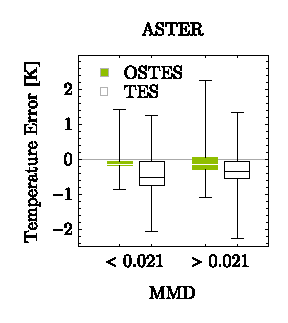
\includegraphics[scale=1]{pics/Chapter_04/Simulated_data_ASTER.eps}
		\caption{}
	\end{subfigure}
	\hspace{1em}
	\begin{subfigure}[t]{.3\linewidth}
		\centering
		\includegraphics[scale=1]{pics/Chapter_04/Simulated_data_AHS.eps}
		\caption{}
	\end{subfigure}
	\hspace{1em}
	\begin{subfigure}[t]{.3\linewidth}
		\centering
		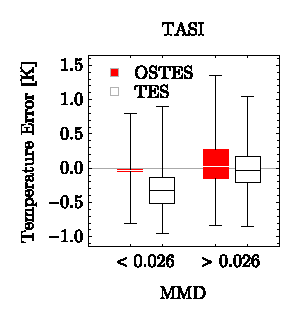
\includegraphics[scale=1]{pics/Chapter_04/Simulated_data_TASI.eps}
		\hspace{1cm}\caption{}
	\end{subfigure}
	\vspace{1.5 em}
	\caption{Box plots representing temperature error produced by OSTES and TES algorithm for ASTER, AHS and TASI sensor. Results are divided in two groups based on the Maximum-Minimum emissivity Difference (MMD) in order to demonstrate the improvement of the OSTES algorithm. Whiskers represent minimum and maximum of temperature error.}
	\label{fig:SimualtedDataTemperatureErrorVsLowVsHighMMD}
\end{figure}

Note that the temperature retrievals using OSTES are both more accurate and more precise than TES in the case of samples with low spectral contrast. It is also important to note that no significant improvement is evident for samples with higher spectral contrast. 

Let us remind the reader that every sample is processed under several different atmospheric conditions coupled with different sample temperatures. Thus the standard deviation of temperature and emissivity error is indicative of the algorithm's sensitivity to seasonal fluctuations. A comparison of standard deviations of temperature errors introduced by both TES approaches reveals that the OSTES is less sensitive to changes in atmosphere and sample temperature for samples with low MMD. However, the standard deviations of temperature errors of samples with higher MMD are similar. Standard deviations of temperature errors obtained by the OSTES and TES algorithms are summarized in the Table \ref{table:StandardDeviations}.

\section{Comparison with ASTER standard products}

The OSTES temperature and emissivity were compared with ASTER standard products AST\_08 (kinetic temperature) and AST\_05 (surface emissivity). For this purpose were chosen scenes containing water bodies. Water emissivity is well-known and does not vary significantly which offers a unique opportunity for testing various algorithm features. Water bodies are commonly used for calibration \cite{TP05-2,T05} and validation \cite{TP05, TP01} purposes.

\begin{table}[!t]
\vspace{0.5em}
\footnotesize
\centering
\begin{tabular}{cccc}
\toprule
Sensor & MMD & OSTES & TES \\ \hline
ASTER 	& $< 0.021$ & 0.25 & 0.50 \\
 		& $> 0.021$ & 0.36 & 0.43 \\ \hline
AHS 		& $< 0.052$ & 0.13 & 0.20 \\
 		& $> 0.052$ & 0.20 & 0.19 \\ \hline
TASI 	& $< 0.026$ & 0.16 & 0.32 \\
 		& $> 0.026$ & 0.32 & 0.30 \\
\bottomrule
\end{tabular}
\vspace{1.5 em}
\caption{Standard deviations of temperature errors obtained by applying OSTES and TES algorithm on simulated data as seen by ASTER, AHS and TASI grouped according to the sample Maximum-Minimum emissivity Difference (MMD). }
\label{table:StandardDeviations}
\normalsize
\end{table}

Testing was focused on: 1) investigating the impact of  various atmospheric conditions on emissivity retrievals of the same material, and 2) emissivity smoothness over homogeneous areas. Both tests were performed on ASTER scenes containing large water bodies, since water emissivity is well-known. For the first test we chose five scenes of the Caspian Sea acquired in various seasons of the year. For the second test we chose Lake Baikal. The list of all scenes used, together with their acquisition and processing dates, is given in Table \ref{table:ASTERScenes}. For every scene we downloaded ASTER standard products AST\_09T, AST\_08 and AST\_05 delivering land-leaving and downwelling radianace, surface kinetic temperature and surface emissivity, respectively. Product AST\_09T was used as input to the OSTES algorithm. The resulting temperatures and emissivities were then compared with the AST\_08 and AST\_05 standard products. The emissivity variability over large and homogeneous water bodies was chosen to be the quality indicator, since we are interested in the retrieval of material properties, which should be essentially constant over time and space.

\begin{table}[!t]
\vspace{0.5em}
\footnotesize
\centering
\begin{tabular}{cccc}
\toprule Location & Acq date (UTC) & Processing date & \parbox[c][1.4cm][c]{1.8cm}{\centering { Precipitable \\ water \\ $\mathrm{[kg\,m^{-3}]}$}} \\ \hline
Caspian Sea & 11.02.2001 - 07:35:55 & 19.11.2015 &  { 9} \\
Caspian Sea & 29.06.2002 - 07:31:47 & 19.11.2015 &  {30} \\
Caspian Sea & 21.08.2004 - 07:29:35 & 19.11.2015 &  {21} \\
Caspian Sea & 30.09.2001 - 07:35:57 & 19.11.2015 &  {28} \\
Caspian Sea & 13.11.2008 - 07:24:21 & 19.11.2015 &  {10} \\
Lake Baikal & 22.07.2002 - 04:17:29 & 27.08.2015 &  {18} \\

\bottomrule
\end{tabular}
\vspace{1.5 em}
\caption{ASTER scenes used for algorithm testing}
\label{table:ASTERScenes}
\normalsize
\end{table}

\subsection*{Caspian Sea}

From the Caspian Sea scenes we chose samples of size $40 \times 40$ pixels over uniform, cloudless waterbody. These subsets were processed by the OSTES algorithm and the emissivity results were averaged for every scene. The results are plotted in Figure \ref{fig:CaspianSeaEmissivity} along with the emissivities that were delivered in the AST\_05 product and averaged over the same spatial subset. In most cases the AST\_05 emissivity spectra appear to be closer to the sea water emissivity spectra taken from ASTER spectral library \cite{BH09}. However, the temperature retrievals of extracted samples obtained by OSTES and TES are very close (not shown). The average temperature difference of AST\_08 and OSTES results computed from all Caspian Sea samples is 0.2\,K (s.d. 0.2\,K). The fact that the temperatures obtained with the two algorithms are very close, but the emissivities are not implies that the emissivity spectra from AST\_05 product are not consistent with temperature from AST\_08 product. We verified this inconsistency by taking the temperatures delivered in AST\_08 and the downwellig and land-leaving radiances delivered in AST\_09T and putting these into (\ref{eq:emissivityComputation}) to obtain emissivities that are different from what is in the AST\_05 product. These emissivity spectra derived from AST\_08 and AST\_09T, which we refer to as ``recomputed emissivities'', are depicted on Figure \ref{fig:CaspianSeaEmissivity} as well. 

Comparison of recomputed emissivity spectra with OSTES emissivity retrievals shows that spectra are nearly identical in scenes acquired on 29.6.2002 and 30.9.2001. Agreement between these emissivity spectra are the consequence of similar AST\_08 and OSTES temperatures; the average difference is \SI{-0.04}{\kelvin} (s.d. \SI{0.15}{\kelvin}). It may be important to note that these scenes contain clouds in part adjacent to the processed sample. On the other hand OSTES results perform slightly better in scenes acquired on 11.2.2001, 21.8.2004 and 13.11.2008. The average temperature difference between AST\_08 and OSTES in these scenes is \SI{0.28}{\kelvin} (s.d. \SI{0.13}{\kelvin}). Nevertheless, none of the emissivity spectra agrees with expected values.

\begin{figure*}[!t]
\centering
\includegraphics[width=0.98\linewidth]{pics/Chapter_04/Caspian.pdf}
\vspace{1.5 em}
\caption{Emissivity of Caspian Sea in different seasons obtained from the ASTER standard product AST\_05, OSTES retrieval, and emissivity recomputation according to the temperature from AST\_08 and land-leaving and downwelling radiance from AST\_09T. Emissivities were extracted from an area of size $40 \times 40$ pixels over pure and cloudless waterbody. Error bars display standard deviation.}
\label{fig:CaspianSeaEmissivity}
\end{figure*}

\begin{figure}[!h]
\centering
\includegraphics[width=0.76\linewidth]{pics/Chapter_04/Baikal.pdf}
\vspace{1.5 em}
\caption{
ASTER band 10 emissivity images of Lake Baikal obtained from ASTER standard product AST\_05 (top) and OSTES emissivity retrieval (middle). In both images the same contrast stretching is used. The white square represents the area from which emissivity histrograms were created (bottom panel). Histograms show distributions of AST\_05 emissivity, OSTES emissivity and recomputed emissivity according to the temperature from AST\_08 and land-leaving and downwelling radiance from AST\_09T. Vertical line depicted in histograms indicates the expected value of water emissivity retrieved from ASTER spectral library \cite{BH09}.}
\label{fig:Bajkal}
\end{figure}

\subsection*{Lake Baikal}

The difference in emissivity obtained by the two versions of TES is further illustrated in the scene over Lake Baikal shown in Figure \ref{fig:Bajkal}. In this figure the white squares on the images define a water body sample of size $90 \times 90$ pixels that was used to produce the values in the histograms below the images. The expected values of sea water emissivity (red vertical line) are included in the Figure \ref{fig:Bajkal}. The histograms show the OSTES emissivity retrievals compared against the AST\_05 standard product, as well as the emissivity recomputed with respect to the temperature delivered by AST\_08 and land-leaving and downwelling radiance delivered by AST\_09T, as described in the previous paragraph. Inspection of the ASTER standard product AST\_05 shows that emissivity values in bands 10, 11 and 12 over the homogeneous study sample are clustered around two distinct values. This creates step discontinuities which are reflected in the bimodal distributions in the histograms and in the noisy patterns in the left image. This will be discussed further below. In contrast to AST\_05 emissivities, OSTES emissivity results are smoother and the histograms do not show any significant bimodality. The recomputed and OSTES emissivity retrievals are similar. However, the OSTES emissivities tend to be closer to the expected values. In addition to the noise, striping is also visible in the image. Striping is caused by electronic noise and can distort emissivity spectra by triggering thresholds included in the original TES algorithm. This can cause step discontinuities. Temperature retrievals are not significantly affected. Striping is more thoroughly discussed in \cite{GA11}. Even though the AST\_05 and OSTES emissivities differ significantly in some bands, the temperature retrievals are very similar. The average difference is \SI{0.25}{\kelvin} (s.d. \SI{0.18}{\kelvin}). Similar to the discussion regarding Caspian Sea emissivity retrievals, it can also be concluded in this case that none of the emissivity spectra have satisfying values.

\begin{figure}[!t]
\centering
\vspace{0.8 em}
\includegraphics[scale=0.85]{pics/Chapter_04/Brno.pdf}
\vspace{2 em}
\caption{
Part of flight line over the city of Brno. Image data were acquired on 4.7.2015 at 14:03 (UTC). The top image displays RGB composition of the studied area. The middle image depicts temperature map obtained from OSTES algorithm applied on image data from TASI sensor. The bottom image is false color emissivity map obtained from OSTES algorithm (red - band 10, green - band 15, blue - band 20). On the top and middle images are shown locations and labels \textit{in-situ} measurements.}
\label{fig:Brno}
\end{figure}

The discrepancies in shape and magnitude of emissivity spectra can be the result of various source of errors but the main error source has been attributed to imperfect atmospheric corrections \cite{TP01, TP05}. Table \ref{table:ASTERScenes} indicates the amount of precipitable water in the atmosphere for each of the investigated scenes. These values were obtained from NOAA's Climate Forecast System Reanalysis. It can be observed that discrepancies in emissivity spectra are related to amount of precipitable water in the atmosphere. Notable works discussing emissivity retrievals over agricultural areas and water bodies are \cite{CC07, SJ07}. One suggested improvement is the water vapour scaling method \cite{T05, GA11}.

The step discontinuities in emissivity values over homogeneous areas can occur due to various thresholds deciding how to treat the sample during processing. The original TES algorithm starts in the NEM module assuming a maximum emissivity spectra $\varepsilon_\mathrm{max}=0.99$. The NEM module is then restarted with refined $\varepsilon_\mathrm{max}$ according to the emissivity retrieved from the first NEM pass. When the NEM iterations do not converge, then the correction for downwelling radiance is not possible, and obtained values of temperature and emissivity are reported as final. The original version of TES processes samples according to the MMD of emissivity spectra obtained from the NEM module either by incorporating (\ref{eq:MMD}) or by presetting emissivity to $\varepsilon = 0.983$. Some authors \cite{GG06}, \cite{SG09} have suggested that the value of the threshold used for classifying observations into groups with either low or high spectral contrast should be changed or completely removed. Observations with wrongly determined spectral contrast or observations with spectral contrast close to any threshold result in step discontinuities. On the contrary, the OSTES does not set any thresholds for materials with low spectral contrast and so it is expected to generate smoother results on homogeneous areas with low spectral contrast.

\section{Application to TASI Image Data}

The OSTES algorithm was applied on image data acquired by TASI sensor and the results were compared with emissivities obtained from \textit{in-situ} mesaurements and the TES algorithm esmissivity estiamtions. 

\subsection*{Experiment Setup}

The study was performed using data acquired over the city of Brno, Czech Republic (lat: 49.2, lon: 16.6). The examined data are subset of a flight line crossing the city from south-west to north-east. The acquisition was performed on 4.7.2015 at 14:03 (UTC). The FLIS operated by Global Change Research Institute CAS (Brno, Czech Republic) \cite{HF14} was used for this acquisition. FLIS consists of Compact Airborne Spectrographic Imager (CASI), Shortwave infrared Airborne Spectrographic Imager (SASI) and TASI sensor. All sensors are developed by Itres Ltd. (Calgary, Canada).

Within this study were performed \textit{in-situ} measurements of urban materials with Fourier transform infrared (FTIR) Spectrometer Models 102 developed by D\&P Instruments (Simsbury, USA). The emissivity of measured surfaces was estimated by a spectral smoothing algorithm \cite{HJ98}. Emissivity spectra of water and deciduous trees were not measured but instead they were extracted from ASTER spectral library \cite{BH09}. All emissivity spectra were resampled with respect to TASI response functions. The study area and locations of the \textit{in-situ} measurements are shown in the upper part of the Figure \ref{fig:Brno}. 

Spectral emissivity libraries are very useful for calibration and validation purposes. Let us emphasize that there are many other spectral emissivity libraries available apart from ASTER spectral library. Notable libraries are Johns Hopkins University Spectral Library \cite{SW91}, Arizona State University Spectral Library \cite{CB00}, United States Geological Survey Spectral Library \cite{CS16} and the Spectral Library of Urban Materials (SLUM) \cite{KS14}. In the Appendix \ref{app:Library} is described a spectral emissivity library which is specifically focused on spoil substrates.

\subsection*{The OSTES implementation to the TASI Processing Chain}

Image data acquired by the TASI sensor were radiometrically, atmospherically and gemetrically pre-processed as described in the Chapter~\ref{chap:Data}. The result of the pre-processing is land-leaving radiance, which is the first input parameter for the OSTES and the TES algorithm. The second input parameter to the both algorithms is downwelling atmospheric radiance. This quantity was obtained from radiative transfer model MODTRAN~\cite{BG06}. The input to MODTRAN requires temperature and water vapour profiles, which were extracted from MOD07\_L2 product~\cite{B11} generated from MODIS image data.

The described procedure of the temperature and emissivity estimation from the pre-processed TASI image data is the continuation of the processing chain introduced in the Chapter~\ref{chap:Data}. The schematic illustration of the OSTES implementation into the processing chain of the TASI image data is depicted in the Figure~\ref{fig:OSTESProcessingChain}, which is the continuation of the processing chain depicted in the Figure~\ref{fig:ProcessingChain}. The whole processing chain of TASI image data described in this work is operational at Global Change Research Institute CAS (Brno, Czech Republic).

\begin{figure}[thb]
	\centering
	\vspace{0.7 em}
	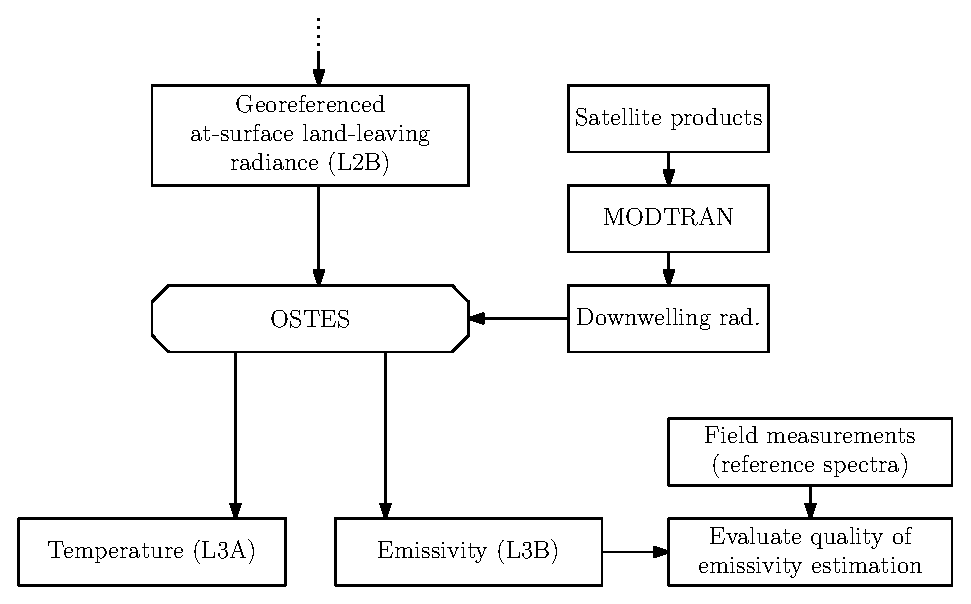
\includegraphics[scale=1]{pics/Chapter_04/OSTES_processing_chain.eps}
	\vspace{2 em}
	\caption{Continuation of the processing chain of the TASI image data introduced in the Chapter \ref{chap:Data} and depicted in the Figure \ref{fig:ProcessingChain}. This part illustrates temperature and emissivity separation processing chain applied to the pre-processed TASI image data.}
	\label{fig:OSTESProcessingChain}
	\vspace{0.7 em}
\end{figure}

The processing of the TASI image data acquired during this experiment was limited to 22 spectral bands. First five and last five spectral bands were not considered since they were affected by imperfect atmospheric corrections.

The TASI image data were processed by the TES and OSTES algorithms in order to~compare the temperature and emissivity retrievals. The TASI image data were processed with the TES algorithm by substituting OSTES algorithm in the processing chain of~TASI image data. The implementation of the TES algorithm is based on the implementation described in~the \cite{JS12} without the $\varepsilon_\mathrm{max}$ refinement for emissivities with low spectral contrast.
 
\subsection*{Comparison}

Temperature and emissivity results of the OSTES algorithm are depicted in the middle and lower part of Figure \ref{fig:Brno} in the form of a temperature and emissivity map. The temperature map shows high temperature differences between vegetated and built areas. Emissivity map is a false color composition (red - band 10, green - band 15, blue - band 20) showing variability of surface materials in the image data.

\newpage
The \textit{in-situ} measurements were not performed during the overflight. Therefore temperature could not be used for the comparison and the validation of the TES and OSTES algorithms. The comparison of the TES and the OSTES algorithms' performance was tested against six emissivities obtained from \textit{in-situ} measurements. Results are shown in the Figure \ref{fig:BrnoEmissivityComparison} below, where error bars display standard deviation. Both TES and OSTES emissivity retrievals are very similar. The OSTES performs slightly better than TES in cases of deciduous trees and Svratka River. However, none of these two spectra agrees with the shape and magnitude of the expected emissivity spectra. These discrepancies can be caused by various sources of errors but the main error source has been attributed to the imperfect atmospheric corrections. Emissivities of the spot 5, asphalt parking lots, retrieved by the TES and OSTES significantly differ from \textit{in-situ} measurement. This shift in magnitude is introduced by the insufficient compensation of the downwelling radiance. This spot is surrounded by buildings, which increase the amount of downwelling radiance. This additional radiance is not included in the atmospheric parameters retrieved from MODTRAN. The rest of the emissivity retrievals are considered to follow \textit{in-situ} measurements well. Let us emphasize the reader that OSTES offers only moderate improvements in emissivity retrievals. These are not possible to observe in this comparison due to the magnitude of the error introduced by the imperfect atmospheric corrections. 

These data were acquired within a campaign focused on detecting urban heat island of the city of Brno. The main goal was determination of parameters affecting temperatures in the city. Preliminary observations are introduced in the Appendix \ref{app:Visualisation}.

\begin{figure}[!t]
\centering
\includegraphics[width=\linewidth]{pics/Chapter_04/Brno-Emissivity-Comparison.pdf}
\vspace{1.5 em}
\caption{Comparison of TES and OSTES emissivity retrievals with emissivities obtained from \textit{in-situ} measurements. Error bars display standard deviation.}
\label{fig:BrnoEmissivityComparison}
\end{figure}


